\section{hp-adaptive methods}





\begin{frame}
\frametitle{Table of contents}

\tableofcontents[currentsection]
\end{frame}





\subsection{Finite Element Method}





\begin{frame}
\frametitle{Finite element method}

\begin{minipage}{.59\textwidth}
  \begin{itemize}
  \item Shape functions form nodal basis
    \begin{align*}
    \varphi_i(x_j) = \delta_{ij} =
    \begin{cases}
    1 & \text{for} ~ i=j \\
    0 & \text{for} ~ i \neq j
    \end{cases}
    \end{align*}
  \item $Q_p$ elements from Lagrange interpolation with degree $p$
  \end{itemize}
  
  \vspace{1em}
  
  \begin{itemize}
  \item Finite element approximation is linear combination of shape functions
    \begin{align*}
    u_{hp}(x) = \sum_i \, u_i \, \varphi_i(x)
    \end{align*}
  \item Coefficients $u_i$ are degrees of freedom
  \end{itemize}
\end{minipage}
\hfill
\begin{minipage}{.4\textwidth}
  \vspace{-1em}
  
  \begin{figure}
  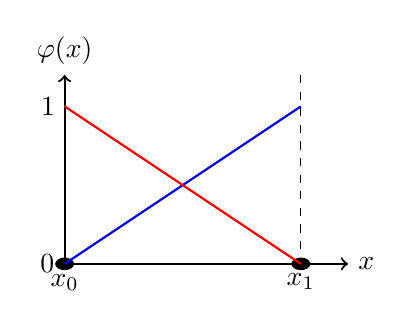
\begin{tikzpicture}[scale=2, xscale=1.5]
  % Draw axes
  \draw [<->,thick] (0,0) node [below] {$x_0$} node[left] {0}
  (0,1.2) node (yaxis) [above] {$\varphi(x)$}
  |- (1.2,0) node (xaxis) [right] {$x$};
  
  % Draw dashed
  \draw [dashed] (1,1.2) -- (1,0) node [below] {$x_1$};
  
  % Draw nodes
  \foreach \x in {0,1} {
    \fill (\x,0) circle (.04cm);
    %\fill (\x,1) circle (.04cm);
  }
  \node[left] at (0,1) {1};
  
  % Draw functions
  \draw[thick,color=blue,domain=0:1] plot (\x,{\x});
  \draw[thick,color=red,domain=0:1] plot (\x,{1-\x});
  \end{tikzpicture}
  \vspace{-0.8em}
  \caption{$Q_1$ element}
  \end{figure}
  
  \vspace{-2.5em}
  
  \begin{figure}
  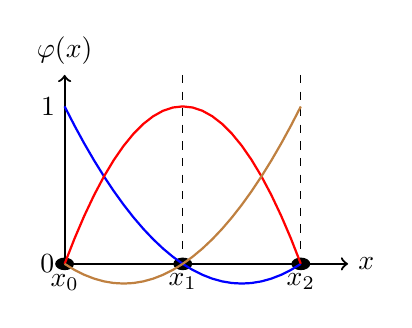
\begin{tikzpicture}[scale=2, xscale=1.5]
  % Draw axes
  \draw [<->,thick] (0,0) node [below] {$x_0$} node[left] {0}
  (0,1.2) node (yaxis) [above] {$\varphi(x)$}
  |- (1.2,0) node (xaxis) [right] {$x$};
  
  % Draw dashed
  \draw [dashed] (0.5,1.2) -- (0.5,0) node [below] {$x_1$};
  \draw [dashed] (1,1.2) -- (1,0) node [below] {$x_2$};
  
  % Draw nodes
  \foreach \x in {0,0.5,1} {
    \fill (\x,0) circle (.04cm);
    %\fill (\x,1) circle (.04cm);
  }
  \node[left] at (0,1) {1};
  
  % Draw functions
  \draw[thick,color=blue,domain=0:1] plot (\x,{2*\x*\x - 3*\x + 1});
  \draw[thick,color=red,domain=0:1] plot (\x,{(-4)*\x*\x + 4*\x});
  \draw[thick,color=brown,domain=0:1] plot (\x,{2*\x*\x - \x});
  \end{tikzpicture}
  \vspace{-0.8em}
  \caption{$Q_2$ element}
  \end{figure}
\end{minipage}
\end{frame}





\subsection{Adaptive methods}





\begin{frame}
\frametitle{Adaptive methods}

\begin{itemize}
\item Focus computational resources on areas of interest
\item Align simulation resolution with complexity of current solution
\end{itemize}

\vfill{}

\begin{itemize}
\item Finite Element Method (FEM) provides two different possibilities:
\begin{tabular}{lll}
  \textbf{\h}-adaptation: & dynamic cell sizes & good for irregular solutions \\
  \textbf{\p}-adaptation: & dynamic function spaces & good for smooth solutions
\end{tabular}
\item Combination of both possible
\end{itemize}

\vfill{}

\begin{minipage}{.49\textwidth}
  \begin{figure}
  \begin{tikzpicture}[scale=2.2]
  \def\Length{0.5}
  \def\Radius{0.03}
  
  \LagrangeCell{-2*\Length}{0}{2*\Length}{\Radius}{2}
  {{,,,,,,,,}};
  
  % remove face node which becomes a hanging node on a vertex
  \draw[fill=white,draw=white] (0,\Length-\Radius) rectangle (-\Radius,\Length+\Radius);
  
  \LagrangeCell{0}{0}{\Length}{\Radius}{2}
  {{,,,,,,,,}};
  \LagrangeCell{\Length}{0}{\Length}{\Radius}{2}
  {{,,,,,,,,}};
  \LagrangeCell{0}{\Length}{\Length}{\Radius}{2}
  {{,,,,,,,,}};
  \LagrangeCell{\Length}{\Length}{\Length}{\Radius}{2}
  {{,,,,,,,,}};
  \end{tikzpicture}
  \caption{\h-adaptivity}
  \end{figure}
\end{minipage}
\begin{minipage}{.49\textwidth}
  \begin{figure}
  \begin{tikzpicture}[scale=2.2]
  \def\Length{1}
  \def\Radius{0.03}
  
  \LagrangeCell{0}{0}{\Length}{\Radius}{2}
  {{,,,,,,,,}};
  \LagrangeCell{\Length}{0}{\Length}{\Radius}{4}
  {{,,,,,,,,,,,,,,,,,,,,,,,,}};
  \end{tikzpicture}
  \caption{\p-adaptivity}
  \end{figure}
\end{minipage}
\end{frame}





\begin{frame}
\frametitle{Adaptation criteria}

\begin{itemize}
\item \textbf{Which} cells to adapt?
\item \textbf{How} to adapt? \h/\p?
\end{itemize}

\pause
\vfill{}

\begin{itemize}
\item Manual adaptation
\item Automatic adaptation
  \begin{itemize}
  \item Criterion to indicate adaptation
  \item General approach -OR- tied to the problem
  \end{itemize}
\end{itemize}

\pause
\vfill{}

\begin{itemize}
\item Automatic \hp-decision strategies discussed in the dissertation
  \begin{enumerate}
  \item Error prediction based on refinement history \newline \parencite{melenk2001}
  \item Smoothness estimation by decay of Fourier coefficients \newline \parencite{bangerth2009}
  \item Smoothness estimation by decay of Legendre coefficients \newline \parencite{mavriplis1994}
  \end{enumerate}
\end{itemize}
\end{frame}





\subsection{Example: Laplace equation}





\begin{frame}
\frametitle{Example: Reentrant corner}

\begin{minipage}{.47\textwidth}
\begin{itemize}
  \item Singularity at reentrant corners for elliptic problems
  \item L-shaped domain:
    \begin{align*}
    \Omega = [-1,1]^2 \setminus \left([0,1]\!\times\![-1,0]\right)
    \end{align*}
  \item Manufactured Laplace problem
    \begin{align*}
    - \nabla^2 u &= 0 \qquad\text{on}\quad \Omega \\
    u &= \bar{u} \qquad\text{on}\quad \partial\Omega \\[.5em]
    \bar{u} &= r^{2/3} \, \sin\left(2/3 ~ \varphi\right) \\
    \|\nabla \bar{u}\| &= r^{-1/3}
    \end{align*}
\end{itemize}
\end{minipage}
\hfill{}
\begin{minipage}{.51\textwidth}
  \begin{figure}
  \resizebox{\textwidth}{!}{
    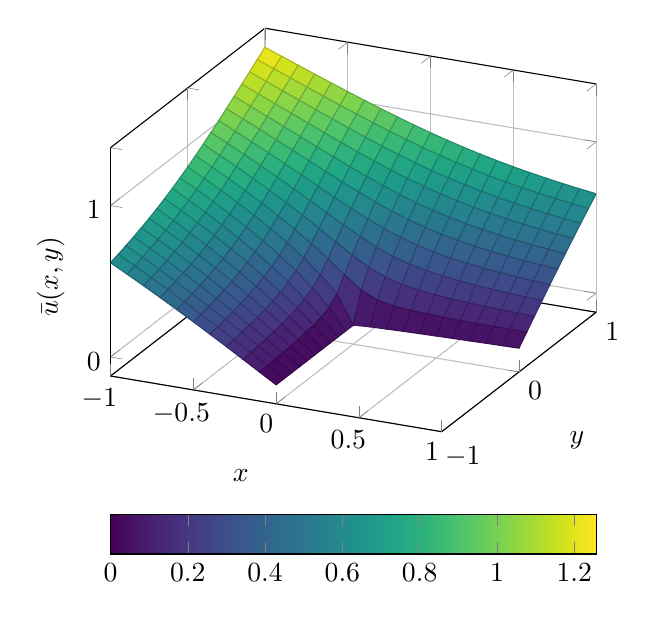
\begin{tikzpicture}
    \begin{axis}[
    scale=0.9,
    grid=major,
    colorbar horizontal,
    colormap/viridis,
    xlabel=$x$,
    ylabel=$y$,
    zlabel={$\bar{u}(x,y)$}
    ]
    \addplot3[
    surf,
    domain=-1:1,
    y domain=-1:1,
    restrict expr to domain={(x>0)&&(y<0)}{0:0},
    samples=21
    ]{pow(x*x+y*y,0.33)*sin(0.66*(atan2(y,-x)+90)))};
    \end{axis}
    \end{tikzpicture}
  }
  \caption{L-shaped domain}
  \end{figure}
\end{minipage}
\end{frame}





\begin{frame}
\frametitle{Example: Successive refinement}

\begin{itemize}
\item Initialize coarse mesh
\item Solve and refine in multiple cycles for tailored discretization
\end{itemize}

\begin{figure}
\begin{tikzpicture}[block/.style={draw}]%, node distance=.35cm]
\node [block] (solve) {SOLVE};
\node [block, right=of solve] (estimate) {ESTIMATE};
\node [block, right=of estimate] (mark) {MARK};
\node [block, right=of mark] (refine) {REFINE};

\draw[->] (solve) -- (estimate);
\draw[->] (estimate) -- (mark);
\draw[->] (mark) -- (refine);
\draw[->] (refine) -- ($ (refine) + (0,-0.8) $)  -| (solve);
\end{tikzpicture}
\caption{Successive refinement}
\end{figure}

\begin{enumerate}
\item Calculate refinement criteria (here: error estimates)
\item Flag 30\%/3\% of cells with highest/lowest criterion for refinement/coarsening
\item Calculate decision criteria (here: smoothness estimates)
\item Flag 90\%/10\% for $p$-/$h$-adaptation
\end{enumerate}
\end{frame}





\begin{frame}
\frametitle{Example: Successive refinement}

\begin{figure}
\only<1>{
  \begin{tikzpicture}
  \begin{axis}[
  scale=1,
  xmin=-1,xmax=1,
  ymin=-1,ymax=1,
  unit vector ratio={1 1},
  tick align=outside,
  xlabel=$x$,
  ylabel=$y$,
  colormap/OrRd,
  colorbar sampled,
  colorbar style={ylabel={finite element polynomial degree}, samples=7, ytick={2,3,...,7}},
  colormap access=piecewise const,
  point meta min=1.5,
  point meta max=7.5
  ]
  
  \addplot graphics [
  xmin=-1,xmax=1,
  ymin=-1,ymax=1,
  ] {illustrations/corner-fedegrees-legendre-00.pdf};
  \end{axis}
  \end{tikzpicture}
  
  \caption{Polynomial degrees in cycle 0. Zoom 100\%.}
}
\only<2>{
  \begin{tikzpicture}
  \begin{axis}[
  scale=1,
  xmin=-1,xmax=1,
  ymin=-1,ymax=1,
  unit vector ratio={1 1},
  tick align=outside,
  xlabel=$x$,
  ylabel=$y$,
  colormap/OrRd,
  colorbar sampled,
  colorbar style={ylabel={finite element polynomial degree}, samples=7, ytick={2,3,...,7}},
  colormap access=piecewise const,
  point meta min=1.5,
  point meta max=7.5
  ]
  
  \addplot graphics [
  xmin=-1,xmax=1,
  ymin=-1,ymax=1,
  ] {illustrations/corner-fedegrees-legendre-01.pdf};
  \end{axis}
  \end{tikzpicture}
  
  \caption{Polynomial degrees in cycle 1. Zoom 100\%.}
}
\only<3>{
  \begin{tikzpicture}
  \begin{axis}[
  scale=1,
  xmin=-1,xmax=1,
  ymin=-1,ymax=1,
  unit vector ratio={1 1},
  tick align=outside,
  xlabel=$x$,
  ylabel=$y$,
  colormap/OrRd,
  colorbar sampled,
  colorbar style={ylabel={finite element polynomial degree}, samples=7, ytick={2,3,...,7}},
  colormap access=piecewise const,
  point meta min=1.5,
  point meta max=7.5
  ]
  
  \addplot graphics [
  xmin=-1,xmax=1,
  ymin=-1,ymax=1,
  ] {illustrations/corner-fedegrees-legendre-02.pdf};
  \end{axis}
  \end{tikzpicture}
  
  \caption{Polynomial degrees in cycle 2. Zoom 100\%.}
}
\only<4>{
  \begin{tikzpicture}
  \begin{axis}[
  scale=1,
  xmin=-1,xmax=1,
  ymin=-1,ymax=1,
  unit vector ratio={1 1},
  tick align=outside,
  xlabel=$x$,
  ylabel=$y$,
  colormap/OrRd,
  colorbar sampled,
  colorbar style={ylabel={finite element polynomial degree}, samples=7, ytick={2,3,...,7}},
  colormap access=piecewise const,
  point meta min=1.5,
  point meta max=7.5
  ]
  
  \addplot graphics [
  xmin=-1,xmax=1,
  ymin=-1,ymax=1,
  ] {illustrations/corner-fedegrees-legendre-03.pdf};
  \end{axis}
  \end{tikzpicture}
  
  \caption{Polynomial degrees in cycle 3. Zoom 100\%.}
}
\only<5>{
  \begin{tikzpicture}
  \begin{axis}[
  scale=1,
  xmin=-1,xmax=1,
  ymin=-1,ymax=1,
  unit vector ratio={1 1},
  tick align=outside,
  xlabel=$x$,
  ylabel=$y$,
  colormap/OrRd,
  colorbar sampled,
  colorbar style={ylabel={finite element polynomial degree}, samples=7, ytick={2,3,...,7}},
  colormap access=piecewise const,
  point meta min=1.5,
  point meta max=7.5
  ]
  
  \addplot graphics [
  xmin=-1,xmax=1,
  ymin=-1,ymax=1,
  ] {illustrations/corner-fedegrees-legendre-04.pdf};
  \end{axis}
  \end{tikzpicture}
  
  \caption{Polynomial degrees in cycle 4. Zoom 100\%.}
}
\only<6>{
  \begin{tikzpicture}
  \begin{axis}[
  scale=1,
  xmin=-1,xmax=1,
  ymin=-1,ymax=1,
  unit vector ratio={1 1},
  tick align=outside,
  xlabel=$x$,
  ylabel=$y$,
  colormap/OrRd,
  colorbar sampled,
  colorbar style={ylabel={finite element polynomial degree}, samples=7, ytick={2,3,...,7}},
  colormap access=piecewise const,
  point meta min=1.5,
  point meta max=7.5
  ]
  
  \addplot graphics [
  xmin=-1,xmax=1,
  ymin=-1,ymax=1,
  ] {illustrations/corner-fedegrees-legendre-05.pdf};
  \end{axis}
  \end{tikzpicture}
  
  \caption{Polynomial degrees in cycle 5. Zoom 100\%.}
}
\only<7>{
  \begin{tikzpicture}
  \begin{axis}[
  scale=1,
  xmin=-0.5,xmax=0.5,
  ymin=-0.5,ymax=0.5,
  unit vector ratio={1 1},
  tick align=outside,
  xlabel=$x$,
  ylabel=$y$,
  colormap/OrRd,
  colorbar sampled,
  colorbar style={ylabel={finite element polynomial degree}, samples=7, ytick={2,3,...,7}},
  colormap access=piecewise const,
  point meta min=1.5,
  point meta max=7.5
  ]
  
  \addplot graphics [
  xmin=-1,xmax=1,
  ymin=-1,ymax=1,
  ] {illustrations/corner-fedegrees-legendre-05.pdf};
  \end{axis}
  \end{tikzpicture}
  
  \caption{Polynomial degrees in cycle 5. Zoom 200\%.}
}
\only<8>{
  \begin{tikzpicture}
  \begin{axis}[
  scale=1,
  xmin=-0.25,xmax=0.25,
  ymin=-0.25,ymax=0.25,
  unit vector ratio={1 1},
  tick align=outside,
  xlabel=$x$,
  ylabel=$y$,
  colormap/OrRd,
  colorbar sampled,
  colorbar style={ylabel={finite element polynomial degree}, samples=7, ytick={2,3,...,7}},
  colormap access=piecewise const,
  point meta min=1.5,
  point meta max=7.5
  ]
  
  \addplot graphics [
  xmin=-1,xmax=1,
  ymin=-1,ymax=1,
  ] {illustrations/corner-fedegrees-legendre-05.pdf};
  \end{axis}
  \end{tikzpicture}
  
  \caption{Polynomial degrees in cycle 5. Zoom 400\%.}
}
\only<9>{
  \begin{tikzpicture}
  \begin{axis}[
  scale=1,
  xmin=-0.125,xmax=0.125,
  ymin=-0.125,ymax=0.125,
  scaled x ticks = false,
  x tick label style={/pgf/number format/fixed},
  scaled y ticks = false,
  y tick label style={/pgf/number format/fixed},
  unit vector ratio={1 1},
  tick align=outside,
  xlabel=$x$,
  ylabel=$y$,
  colormap/OrRd,
  colorbar sampled,
  colorbar style={ylabel={finite element polynomial degree}, samples=7, ytick={2,3,...,7}},
  colormap access=piecewise const,
  point meta min=1.5,
  point meta max=7.5
  ]
  
  \addplot graphics [
  xmin=-1,xmax=1,
  ymin=-1,ymax=1,
  ] {illustrations/corner-fedegrees-legendre-05.pdf};
  \end{axis}
  \end{tikzpicture}
  
  \caption{Polynomial degrees in cycle 5. Zoom 800\%.}
}
\end{figure}
\end{frame}





\begin{frame}
\frametitle{Example: Successive refinement}

\begin{minipage}{1.08\textwidth}
  \begin{figure}
    \hspace{-1cm}
    \begin{subfigure}{.32\textwidth}
    \centering
    \begin{tikzpicture}
    \begin{axis}[
    scale=0.72,
    xmin=-1,xmax=1,
    ymin=-1,ymax=1,
    ticks=none,
    unit vector ratio={1 1},
    ]
    
    \addplot graphics [
    xmin=-1,xmax=1,
    ymin=-1,ymax=1,
    ] {illustrations/corner-fedegrees-fourier-05.pdf};
    \end{axis}
    \end{tikzpicture}
    \caption{Fourier coefficient decay}
    \end{subfigure}
    \begin{subfigure}{.32\textwidth}
    \centering
    \begin{tikzpicture}
    \begin{axis}[
    scale=0.72,
    xmin=-1,xmax=1,
    ymin=-1,ymax=1,
    ticks=none,
    unit vector ratio={1 1},
    ]
    
    \addplot graphics [
    xmin=-1,xmax=1,
    ymin=-1,ymax=1,
    ] {illustrations/corner-fedegrees-legendre-05.pdf};
    \end{axis}
    \end{tikzpicture}
    \caption{Legendre coefficient decay}
    \end{subfigure}
    \begin{subfigure}{.32\textwidth}
    \centering
    \begin{tikzpicture}
    \begin{axis}[
    scale=0.72,
    xmin=-1,xmax=1,
    ymin=-1,ymax=1,
    ticks=none,
    unit vector ratio={1 1},
    ]
    
    \addplot graphics [
    xmin=-1,xmax=1,
    ymin=-1,ymax=1,
    ] {illustrations/corner-fedegrees-prediction-05.pdf};
    \end{axis}
    \end{tikzpicture}
    \caption{Refinement history}
  \end{subfigure}
  \caption{Mesh and polynomial degrees of finite elements after 5 consecutive \newline $hp$-adaptations.}
  \end{figure}
\end{minipage}
\end{frame}




\begin{frame}
\frametitle{Example: Successive refinement}

\begin{figure}
\begin{tikzpicture}
\begin{loglogaxis}[
scale=1,
xlabel={Number of degrees of freedom},
ylabel={H1 error},
grid=major,
legend cell align=left,
legend pos=outer north east,
]
\addplot table [y=H1 error, x=ndofs, col sep=comma] {data/error/hp-legendre.csv};
\addlegendentry{\hp{} Legendre};

\addplot table [y=H1 error, x=ndofs, col sep=comma] {data/error/hp-fourier.csv};
\addlegendentry{\hp{} Fourier};

\addplot table [y=H1 error, x=ndofs, col sep=comma] {data/error/hp-prediction.csv};
\addlegendentry{\hp{} prediction};

\addplot table [y=H1 error, x=ndofs, col sep=comma] {data/error/h.csv};
\addlegendentry{\h};
\end{loglogaxis}
\end{tikzpicture}
\caption{Error convergence for different strategies}
\end{figure}
\end{frame}